
\newcommand{\pderiv}[2]{\frac{\partial #1}{\partial #2}}
\newcommand{\pderivv}[2]{\frac{\partial^2 #1}{\partial #2 ^2}}

% setup paths for images
%\graphicspath{ {images/} }


% define the title and authors that will be used in the report
\title{ Homework 1 \\ CS 544 - Optimization in Computer Vision }
\author{
	% Sugar & Caffeine
	Christian Howard \\ howard28@illinois.edu
	\and
	Patrick Zhai \\ haoyuz5@illinois.edu
	\and
	Rishika Agarwal \\ rishika2@illinois.edu
	\and
	Yuxuan Zhou \\ yuxuanz6@illinois.edu
}

% start the document
\begin{document}
\maketitle

\section{Introduction}
Optimization is a crucial part to modern day computing. Numerical Optimization is not limited to familiar domains of statistical modeling and Machine Learning, but also finds itself being used in everything from Design Optimization in engineering to Optimal Control and Guidance systems on missiles, solving nonlinear equations modeling physical systems, and plenty more. Investigating the characteristics of different optimization techniques is crucial for ensuring we apply them to appropriate problems. Within this report we investigate two techniques, namely:

\begin{enumerate}
    \item Quasi-Newton using Conjugate Gradient \label{qncq}
    \item Nonlinear Conjugate Gradient using Polak-Ribiere update \label{pr}
\end{enumerate}

We will start the analysis by considering a toy problem that will allow us to readily investigate numerical properties of the two techniques, and some variations of them, in a variety of contexts. Following this, we will see how the two methods contrast each other across some case study problems within the context of classification in Machine Learning. 

\newpage
\section{Analysis using Toy Problem}
\subsection{Intro}
When considering the two optimization techniques given in \ref{qncq} and \ref{pr}, both techniques clearly make their estimates for the optimum of a problem using different sets of information. The Quasi-Newton method benefits with explicit curvature information while the Polak-Ribiere flavor of Nonlinear Conjugate Gradient attempts to advance optimum estimates using conjugate directions and then performing line searches to advance as far as possible along proposed descent directions. While Quasi-Newton gets more information, it also requires a heftier computational cost to obtain the desired search direction. 

This trade-off is ultimately where one can see situations where one method might prove superior to the other. To gain some further insight, we will investigate the below toy problem.

\begin{align}
    &\min_{\bv{x} \Real^d} &&g_{\alpha}(\bv{x}) = (1-\alpha) f_1(x) + \alpha f_2(x) \label{toy}\\
    &\text{where } &&f_1(\bv{x}) = \sum_{k=1}^d \left(x_k\right)^2 \nonumber \\
    & &&f_2(\bv{x}) = \sum_{k=1}^d \left(x_k\right)^4 \nonumber
\end{align}

We will vary this toy problem for different values of problem dimension $d$, as well as vary $\alpha \in [0,1]$ to perform a convex combination of the two convex functions $f_1$ and $f_2$. This toy problem gives us analysis benefits with a known global optimal solution at $\bv{x}^* = \bv{0}$ as well as makes it simple to investigate how the dimensionality of the problem and the variation in second derivative magnitudes as a function of state impacts convergence.

\subsection{Analysis}
Within this analysis, we investigate differences in performance between Full Quasi-Newton, Sparse Quasi-Newton, the vanilla Polak-Ribiere method, and the Polak-Ribiere method with Restart executed against the toy problem defined in \eqref{toy}. The Full Quasi-Newton is the Conjugate Gradient based Quasi-Newton method such that it uses the full, dense Hessian matrix. The Sparse Quasi-Newton method is similar but instead uses a sparse representation and matrix-vector product (matvec) form of the Hessian for use in the Conjugate Gradient algorithm.

We perform our analysis using values $\alpha \in \lbrace 0, 0.25, 0.5, 0.75, 1 \rbrace$ and $d \in d_{low} \cup d_{high}$, where $d_{low} = \lbrace 10, 50, 100 \rbrace$ is the set of low dimension test values, and $d_{high} = \lbrace 1000, 2000, 3000 \rbrace$ is the set of high dimension test values. The initial condition is set to $\bv{x}_0 &= \bv{2}$ so that we can start off with reasonably large second derivative values as $\alpha$ gets large. Further, convergence for this problem is defined as when $\norm{\nabla_{x} g_{\alpha}(\bv{x})}_{\infty} \leq \tau$ for $\tau = 10^{-6}$. Using this criteria, Figures \ref{fig:low_fqn} through \ref{fig:high_pr} represent the number of iterations and run-time results for different values of $\alpha$ and $d$ for each of the three methods.

Looking at Figures \ref{fig:low_fqn} through \ref{fig:high_prr}, there are some clear trends between the various methods. Consistently, the run-time performance across both low and high dimensional problems shows that Sparse Quasi-Newton converges in a shorter run-time than the Polak-Ribiere methods, while the Polak-Ribiere methods converge in a shorter run-time than the Full Quasi-Newton. In the low dimensional cases, the time differences are small between the various methods but for high dimensional problems, Sparse Quasi-Newton is an order of magnitude faster than Polak-Ribiere, which is also an order of magnitude faster than the Full Quasi-Newton.

Both Quasi-Newton approaches converge in few iterations relative to the Polak-Ribiere methods, but the Full Quasi-Newton method does more work per iteration than Polak-Ribiere, which ultimately explains why the Full Quasi-Newton method is slower than the Polak-Ribiere techniques. Since the Sparse Quasi-Newton method performs fast matvec operations within the Conjugate Gradient solver, its run-time is significantly smaller than the Full Quasi-Newton counterpart. Couple that with the few iterations, it seems reasonable why the Sparse Quasi-Newton technique shows superior performance relative to the Polak-Ribiere techniques. Interestingly, the restart flavor of Polak-Ribiere appears to perform similarly to the vanilla Polak-Ribiere technique in all the results seen in the analysis. It appears the toy problem might not have the properties needed to really see the pros and cons of using the restart technique or not.

Some other interesting things to note is the performance affects of changing $(\alpha,d)$. For the Quasi-Newton methods, there is a clear increase in run-time and number of iterations as the second derivative magnitudes, and their variation, increase. This trend holds for all $d$, generally speaking. For the Polak-Ribiere method, we see some generally increasing run-time and number of iterations as the second derivative magnitudes increase. However, for $d = 100$ we see some peculiar behavior where $\alpha = 0.25$ took the longest in both run-time and number of iterations. Reasons for this are not clear but suspicion lies with the choices of approximate line search technique. 

Another interesting observation is that for the Quasi-Newton methods, the number of iterations they took was identical for all values of $d$, given some $\alpha$. This observation seems to be due to the explicit use of curvature information and how this information transcends the number of dimensions for this toy problem. Polak-Ribiere, on the other hand, displayed variation in the number of iterations it requires for different values of $(\alpha,d)$, which was interesting. This showed us that the conjugate directions coupled with the line search really influence the convergence in a dimension and curvature dependent manner.

\begin{figure}[h!]
    % full quasi-newton
    \begin{subfigure}{\textwidth}
      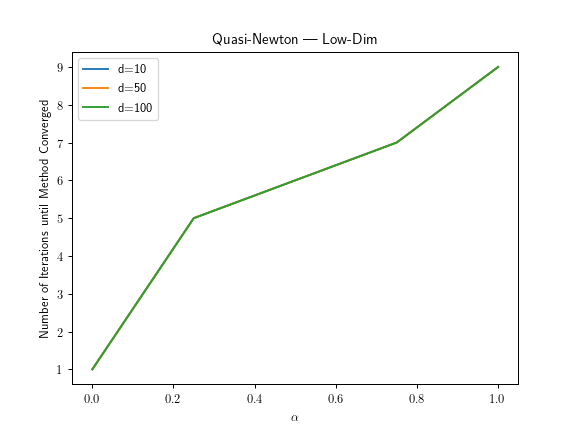
\includegraphics[width=.5\linewidth]{hw1_imgs/qn_low_iter}\hfill
      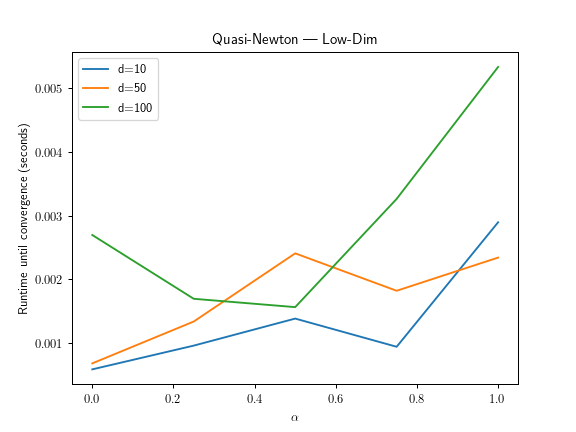
\includegraphics[width=.5\linewidth]{hw1_imgs/qn_low_rt}
      \caption{$(\alpha,d_{low})$-study: Number of iterations until convergence (left) and Run-time until convergence (right) using \textit{Full Quasi-Newton}}
      \label{fig:low_fqn}
    \end{subfigure}%
    % sparse quasi-newton
    \begin{subfigure}{\textwidth}
      \includegraphics[width=.5\linewidth]{hw1_imgs/qn_matvec_low_iter}\hfill
      \includegraphics[width=.5\linewidth]{hw1_imgs/qn_matvec_low_rt}
      \caption{$(\alpha,d_{low})$-study: Number of iterations until convergence (left) and Run-time until convergence (right) using \textit{Sparse Quasi-Newton}}
      \label{fig:low_sqn}
    \end{subfigure}%
    % polak-ribiere
    \begin{subfigure}{\textwidth}
      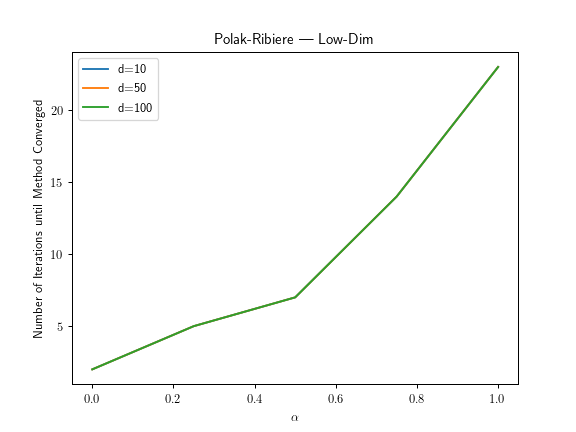
\includegraphics[width=.5\linewidth]{hw1_imgs/pr_low_iter}\hfill
      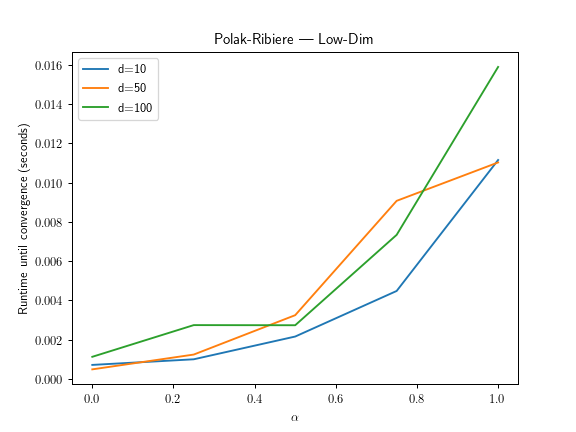
\includegraphics[width=.5\linewidth]{hw1_imgs/pr_low_rt}
      \caption{$(\alpha,d_{low})$-study: Number of iterations until convergence (left) and Run-time until convergence (right) using \textit{Polak-Ribiere}}
      \label{fig:low_pr}
    \end{subfigure}
    % polak-ribiere w/ restart
    \begin{subfigure}{\textwidth}
      \includegraphics[width=.5\linewidth]{hw1_imgs/pr_restart_low_iter}\hfill
      \includegraphics[width=.5\linewidth]{hw1_imgs/pr_restart_low_rt}
      \caption{$(\alpha,d_{low})$-study: Number of iterations until convergence (left) and Run-time until convergence (right) using \textit{Polak-Ribiere with Restart}}
      \label{fig:low_prr}
    \end{subfigure}
\end{figure}


\begin{figure}[h!]
    % full quasi-newton
    \begin{subfigure}{\textwidth}
      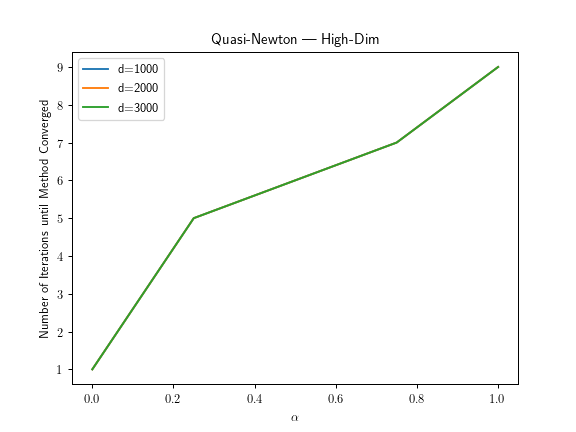
\includegraphics[width=.5\linewidth]{hw1_imgs/qn_high_iter}\hfill
      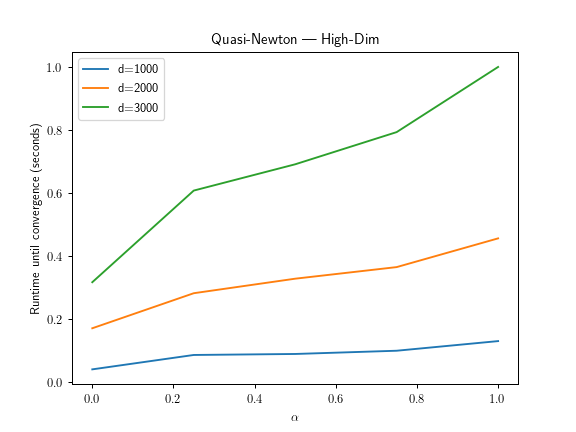
\includegraphics[width=.5\linewidth]{hw1_imgs/qn_high_rt}
      \caption{$(\alpha,d_{high})$-study: Number of iterations until convergence (left) and Run-time until convergence (right) using \textit{Full Quasi-Newton}}
      \label{fig:high_fqn}
    \end{subfigure}%
    % sparse quasi-newton
    \begin{subfigure}{\textwidth}
      \includegraphics[width=.5\linewidth]{hw1_imgs/qn_matvec_high_iter}\hfill
      \includegraphics[width=.5\linewidth]{hw1_imgs/qn_matvec_high_rt}
      \caption{$(\alpha,d_{high})$-study: Number of iterations until convergence (left) and Run-time until convergence (right) using \textit{Sparse Quasi-Newton}}
      \label{fig:high_sqn}
    \end{subfigure}%
    % polak-ribiere
    \begin{subfigure}{\textwidth}
      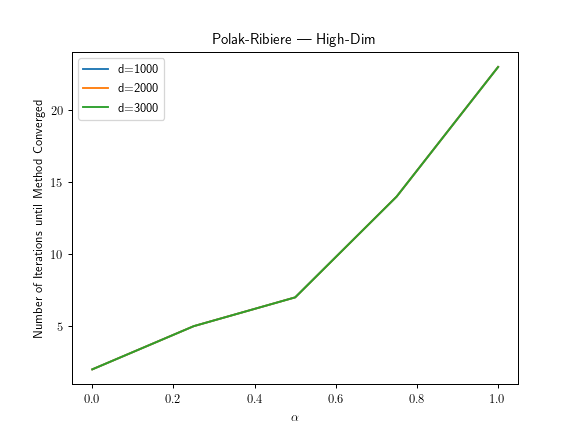
\includegraphics[width=.5\linewidth]{hw1_imgs/pr_high_iter}\hfill
      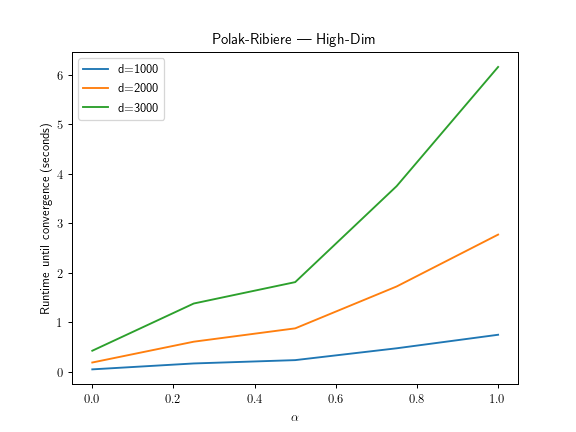
\includegraphics[width=.5\linewidth]{hw1_imgs/pr_high_rt}
      \caption{$(\alpha,d_{high})$-study: Number of iterations until convergence (left) and Run-time until convergence (right) using \textit{Polak-Ribiere}}
      \label{fig:high_pr}
    \end{subfigure}
    % polak-ribiere w/ restart
    \begin{subfigure}{\textwidth}
      \includegraphics[width=.5\linewidth]{hw1_imgs/pr_restart_high_iter}\hfill
      \includegraphics[width=.5\linewidth]{hw1_imgs/pr_restart_high_rt}
      \caption{$(\alpha,d_{high})$-study: Number of iterations until convergence (left) and Run-time until convergence (right) using \textit{Polak-Ribiere with Restart}}
      \label{fig:high_prr}
    \end{subfigure}
\end{figure}

\newpage
\section{Case Studies}
\subsection{Classification with Logistic Regression}
To study the effect of using the two optimization methods for a practical problem, we chose to work with both the MNIST and CIFAR-10 datasets but restrict ourselves to building 1-vs-all classifiers for each dataset. We built a simple regularized logistic regression model based on the principle of classifying images into 2 classes. The probability for $x_i$ belonging to $k^{th}$ class is given by \eqref{eq:prob}. The predicted class label is then the class with the maximum probability.

\begin{align}
p(y_i = k) &= \sigma\left(\beta_{0}^{(k)} + \sum_j \beta_{j}^{(k)} x_j\right) \nonumber \\
&= \frac{1}{1+e^{-(\beta_{0}^{(k)} + \sum_j \beta_{j}^{(k)} x_j)}} \label{eq:prob}
\end{align}

where $\sigma(\cdot)$ is the Sigmoid function, $\beta^{(k)}$ is the parameter vector for class $k$, and $\beta_{j}^{(k)}$ is the $j^{th}$ element of the vector $\beta^{(k)}$. Since we are only working with binary classification, it becomes simple enough to just compute the parameters for $k = 1$ and to use the identity $p(y_i = 0) = 1 - p(y_i = 1)$ to see what the probability is that a digit is \textit{not} $1$. Using this and a negative log-likelihood Maximum Likelihood Estimate approach with some $l_2$ regularization, we obtain the objective function

\begin{align}
    J(\bv{\beta}) &= \frac{-1}{m}\sum_{i=1}^{m} y_i \log\left(\sigma(\bv{\beta}^T \bv{x}_i)\right) + (1 - y_i) \log\left(1 - \sigma(\bv{\beta}^T \bv{x}_i)\right)+ \frac{\lambda}{2 m} \sum_{i=1}^{d} \beta_{i} 
\end{align}

where $D$ is our dataset, $m = |D|$ is our dataset size, $\bv{\beta} \in \Real^{d+1}$ is our parameter vector being estimated, and $\lambda > 0$ is our regularization parameter. In the MNIST dataset, the input images are of size $20\times20$, so $d = 400$ resulting in our optimization taking place in $\Real^{401}$. In the CIFAR-10 dataset, each image is $32 \times 32$ pixels with $3$ color channels, so $d = 3 \times 1024 = 3072$ and in turn makes our optimization take place in $\Real^{3073}$. The regularization hyper-parameter $\lambda$ is kept fixed at $\lambda = 10^{-1}$, so it is not counted as a model parameter.

The summary of the analysis can be found in Figures \ref{fig:mnist1} and \ref{fig:cifar1} as well as Tables \ref{tab:mnist} and \ref{tab:cipar}. The results seen by the collections of figures and tables is actually quite interesting. It is observed that a (Full) Quasi-Newton method based on the Conjugate Gradient method is empirically faster than the Polak-Ribiere method for these Computer Vision classification problems. This is counter-intuitive given the results on the toy problem discussed earlier. 

One noticeable characteristic with this classification problem was that the function evaluations were much more time consuming than in the toy problem since we had to crunch a lot of data for each function evaluation. This influences the speed of the Polak-Ribiere method because it uses a line-search technique that is dependent on numerous function evaluations. Contrasting this to the Quasi-Newton method, the Quasi-Newton method only requires the single construction of the gradient and hessian so that it can find a Quasi-Newton step via Conjugate Gradient, effectively having to work through all the dataset once per iteration. We can model the time complexity of both methods, per iteration, to be the following: 

\begin{align*}
    T_{pr} &= O\left( \underbrace{d}_{\text{Update Conjugate Direction}} + \underbrace{k dm}_{\text{Line Search}} \right) \\
    &= O\left(kdm\right) \\
    T_{qn} &= O\left(\underbrace{md^2}_{\text{Computing gradient and Hessian}} + \underbrace{d^3}_{\text{Conjugate Gradient Solve}}\right) \\
    &= O\left(md^2 + d^3\right)
\end{align*}

where $k$ represents the number of function evaluations needed for the line search. If we assume that $k = O(1)$ and $m \geq d$, we can then find the per-iteration time complexity to be $T_{pr} = O(dm)$ for Polak-Ribiere and $T_{qn} = O(md^2)$ for the (Full) Quasi-Newton method. Clearly, the Quasi-Newton method is slower for large $m$ and $d$ relative to the Polak-Ribiere method. However, if we then take into account that the Quasi-Newton method requires much fewer iterations than the Polak-Ribiere method, one can see how the time complexity of the Polak-Ribiere method could end up being worse overall relative to the Quasi-Newton method, as we observed. In fact, in this empirical situation, it appears the Quasi-Newton method has $O(1)$ number of iterations while the Polak-Ribiere has $O(d)$ iterations, making both methods $O(md^2)$ overall which could help explain the ability for Quasi-Newton to be faster than Polak-Ribiere.

All of this said, it is also important to discuss the trade off in minimizing the objective function too much and overfitting versus stopping early and generalizing better. In fact, the results seen in Figure \ref{fig:cifar1} and Table \ref{tab:cipar} paint an interesting picture. While the Polak-Ribiere method appears to have stalled at a relatively high objective cost relative to the Quasi-Newton method, the test accuracy of the resulting model was better than the Quasi-Newton model. This leads to the obvious conclusion that the Quasi-Newton based model lost its generalization capabilities by minimizing the objective too strongly, even with the presence of some $l_2$ regularization. This presents an interesting problem to consider when applying optimization techniques to Machine Learning problems where ultimately we care about generalization capability instead of finding the exact global minimum of the given objective function.

\begin{minipage}{\linewidth}
\centering
\captionof{table}{MNIST Results} \label{tab:mnist}
\begin{tabular}{l|l l l l|l l l l}
\toprule[1.5pt]
    \bf Method & \bf Iterations & \bf Final Cost & \bf Run-time (s) & \bf Test Accuracy (\%) \\ \hline
    Polak-Ribiere & 211& 0.0188& 11.47& 99\\
    Quasi-Newton & 13& 0.01362& 9.907& 99\\
\bottomrule[1.25pt]
\end{tabular}
\bigskip
\end{minipage}

\begin{minipage}{\linewidth}
\centering
\captionof{table}{CIPAR-10 Results}  \label{tab:cipar}
\begin{tabular}{l|l l l l|l l l l}
\toprule[1.5pt]
    \bf Method & \bf Iterations & \bf Final Cost & \bf Run-time (s) & \bf Test Accuracy (\%) \\ \hline
    Polak-Ribiere & 10,000& 0.1722& 21,240&91\\
    Quasi-Newton & 65& 2.334 \cdot 10^{-4}&3151 &85 \\
\bottomrule[1.25pt]
\end{tabular}
\bigskip
\end{minipage}

\begin{figure}[h!]
    % full quasi-newton
    \begin{subfigure}{\textwidth}
      \includegraphics[width=\linewidth]{hw1_imgs/mnist_out1}\hfill
      \caption{MNIST Objective Function Error vs Iteration Count}
      \label{fig:mnist1}
    \end{subfigure}%
    % sparse quasi-newton
    \begin{subfigure}{\textwidth}
      \includegraphics[width=\linewidth]{hw1_imgs/cifar_out1}\hfill
      \caption{CIFAR-10 Objective Function Error vs Iteration Count}
      \label{fig:cifar1}
    \end{subfigure}
\end{figure}

\section{Conclusion}
After all the studies and analysis completed, there are a few conclusions that can be made. Under the assumption the objective function is cheap to evaluate, Polak-Ribiere methods appears to be good choices to use for low and high dimensional problems alike if you worry about run-time and cannot represent your Hessian at all or in a sparse manner. However, if you can make matrix-vector products with your Hessian matrix fast, then using this with a Quasi-Newton method and the Conjugate Gradient method is ideal for fast convergence and run-time.

Under the assumption the objective function is expensive to evaluate, Quasi-Newton appears to be the winner unless you can find a line search routine that really minimizes function evaluations. In the context of Machine Learning, it appears that requiring the Quasi-Newton to have really small error tolerances could lead to overfitting and so making the tolerances more loose may help to avoid that issue for some fixed regularization.

\newpage
\appendix
\section{Software Implementations}
The optimization routines were implemented in Python with the help of \lstinline{numpy}. Implementations for Linear Conjugate Gradient, Quasi-Newton based on Conjugate Gradient, line search functionality, and Nonlinear Conjugate Gradient with Polak-Ribiere update were all written from scratch using \lstinline{numpy} and used for this assignment. 

The Linear Conjugate Gradient code was designed to allow for specifying a \lstinline{numpy} matrix to solve or a matrix-vector product function/functor that can be used when the matrix is sparse or more efficient to compute via a matrix-vector product. This ability to handle sparse or efficient matvec representations is in turn a feature that the Quasi-Newton optimization procedure can take advantage of if the user desires.

Three line search approaches were implemented. The first was a backtracking line search that aimed to satisfy a sufficient function decrease condition from the Wolfe Conditions. The second was a line search that checks the full Wolfe Conditions and increases the step size estimate each time. The last method used a couple samples of the objective function along the descent direction to construct an approximate model via interpolation. This surrogate model is then minimized to find an approximately optimal step size. 

\comment{
Code for all of the above things can be found below.

\begin{minted}{python}
# line_search.py
import numpy as np

def bt_line_search(f, x, p, alpha_guess=1.0, beta=0.5, c1=1e-4, c2=0.9, maxiter=30):
    # Author: C. Howard
    # This code is doing an approximate line search using
    # backtracking line search

    pmag = np.linalg.norm(p)
    pn = p/pmag
    p[:] = pn[:]

    # compute useful values for when alpha = 0
    out0 = f(x)
    Phi0 = out0[0]
    dPhi0 = np.dot(out0[1],p)

    # if direction is not descent direction
    # then flip the sign of descent dir and slope
    if dPhi0 > 0:
        dPhi0 = -dPhi0
        p[:] = -p[:]

    # define useful functions to compute a good stepsize
    def Phi(alpha):
        return f(x + alpha*p)[0]
    def dPhi_da(alpha):
        return np.dot(f(x + alpha*p)[1],p)
    def condition(alpha):
        return (Phi(alpha) <= (Phi0 + c1*alpha*dPhi0) )

    # define the initial alpha
    alpha = alpha_guess

    # perform inexact line search with armijo rule loop
    iter = 0
    while(iter < maxiter and (not condition(alpha)) ):
        alpha = alpha*beta
        iter = iter + 1

    # return the alpha satisfying the conditions
    #print("alpha: ", alpha)
    return alpha

def wc_line_search(f, x, p, alpha_guess=1e-10, beta=10.0, c1=1e-4, c2=0.9, maxiter=30):
    # Author: C. Howard
    # This code is doing an approximate line search using
    # the Wolf Conditions (as seen in class)

    pmag = np.linalg.norm(p)
    pn = p/pmag
    p[:] = pn[:]

    # compute useful values for when alpha = 0
    out0 = f(x)
    Phi0 = out0[0]
    dPhi0 = np.dot(out0[1],p)

    # if direction is not descent direction
    # then flip the sign of descent dir and slope
    if dPhi0 > 0:
        dPhi0 = -dPhi0
        p[:] = -p[:]

    # define useful functions to compute a good stepsize
    def Phi(alpha):
        return f(x + alpha*p)[0]
    def dPhi_da(alpha):
        return np.dot(f(x + alpha*p)[1],p)
    def condition1(alpha, Phi_a):
        return (Phi(alpha) <= (Phi0 + c1*alpha*dPhi0) )
    def condition2(dPhi_a):
        return (dPhi_a >= (c2*dPhi0))

    # define the initial alpha
    alpha = alpha_guess

    # perform inexact line search with armijo rule loop
    iter = 0
    out = f(x + alpha*p)
    check = condition1(alpha,out[0]) and condition2(np.dot(out[1],p))
    while(iter < maxiter and (not check) ):
        alpha = alpha*beta
        out = f(x + alpha*p)
        check = condition1(alpha,out[0]) and condition2(np.dot(out[1],p))
        iter = iter + 1

    # return the alpha satisfying the conditions
    #print("alpha: ", alpha)
    return alpha

def surrogate_line_search(f, x, p, alpha_guess=100.0, beta=0.5, c1=1e-4, c2=0.9, maxiter=3):
    # Author: C. Howard
    # This code does an approximate line search
    # using surrogate models of the function via
    # interpolation

    pmag = np.linalg.norm(p)
    pn = p/pmag
    p[:] = pn[:]

    # compute useful values for when alpha = 0
    out0 = f(x)
    Phi0 = out0[0]
    dPhi0 = np.dot(out0[1],p)

    # if direction is not descent direction
    # then flip the sign of descent dir and slope
    if dPhi0 > 0:
        dPhi0 = -dPhi0
        p[:] = -p[:]

    # define useful functions to compute a good stepsize
    def Phi(alpha):
        return f(x + alpha*p)[0]
    def dPhi_da(alpha):
        return np.dot(f(x + alpha*p)[1],p)

    # define the initial alpha
    alpha = alpha_guess

    def solve_quadratic(a):
        # compute useful values for alpha_guess
        outg = f(x + a*p)
        A = np.zeros((3,3))
        b = np.zeros((3,))

        # define matrix
        A[0,0:] = [1.0, 0.0, 0.0]
        A[1,0:] = [1.0, a, a**2]
        A[2,0:] = [0, 1.0, 0.0]

        # define the stuff to solve for
        b[:] = [Phi0, outg[0], dPhi0]

        # solve for coefficients
        c = np.linalg.solve(A,b)

        return c

    def surrogate(a, c):
        return c[0] + a*(c[1] + a*c[2])
    def surrogate_d1(a, c):
        return c[1] + a*2.0*c[2]
    def surrogate_d2(a, c):
        return 2.0*c[2]

    # perform minimization using newton
    ag = alpha
    c = solve_quadratic(a=ag)
    d1 = surrogate_d1(ag, c)
    d2 = surrogate_d2(ag, c)
    if d2 != 0.0:
        ag = min(ag/10.0, ag - d1/d2)
    alpha = ag
    
    # return the alpha satisfying the conditions
    #print("alpha: ", alpha)
    return alpha
\end{minted}

\begin{minted}{python}
#conj_grad.py
import numpy as np

def conjugate_gradient(A, b, use_matvec_op = False, epsilon = 1e-12 ):
    # Author: C. Howard
    # Code used to solve linear systems Ax = b
    # for symmetric matrix A based on algorithm described at:
    # https://en.wikipedia.org/wiki/Conjugate_gradient_method
    #
    # [Inputs]
    # A: expected to either be
    #   1) A numpy matrix of dimension n by n for some integer n
    #   2) Some functor/function that takes two input vectors (x, o)
    #      where x is the numpy vector that will have a matvec performed
    #      on it and o is the output numpy vector with the result
    #
    # b: numpy vector
    #
    # use_matvec_op: True if A input is a functor/function representing
    #   matrix-vector multiplications, False if A is a numpy matrix
    #
    # epsilon: Tolerance to check for convergence of algorithm
    #
    # [Outputs]
    # Returns a tuple (x, n) where x is the solution to the system
    # and n is the number of iterations it took to get to that solution

    # define a temporary vector for matvecs
    q = np.zeros(b.shape)

    # define approximate solution
    x = np.zeros(b.shape)

    # construct matvec operator if the one passed
    # in is not a matvec
    if type(A) == np.ndarray:
        def matvec_op(xx, yy):
            np.matmul(A, xx, out=yy)
    else:
        matvec_op = A

    # start the conjugate gradient work
    # by computing initial residual
    matvec_op(x, q)
    r = b - q

    # define function to compute residual error
    def error(r):
        return np.linalg.norm(r, np.inf)

    # check if the solution is good enough
    # with the initial guess and return if so
    resid_err = error(r)
    if resid_err < epsilon:
        return (x,0, resid_err)
    
    # initialize a few useful variables for algo
    max_iters = b.shape[0]
    num_iter = 0
    p = np.copy(r)
    beta = 0.0
    alpha = 0.0

    # loop computing the estimate for the solution
    # until tolerance or max iterations is met
    while (resid_err > epsilon) and (num_iter < max_iters):
        # compute the matvec of A(x) and
        # store in temporary vector
        matvec_op(p,q)

        # compute alpha_{k}
        rmag2 = np.dot(r,r)
        denom = np.dot(p,q)
        if denom > 0: # if this is <= 0, it is not a descent dir
            alpha = rmag2/np.dot(p,q)

            # compute updated solution and residual
            x = x + alpha*p
            r = r - alpha*q
        else:
            #print('problem with bad direction!')
            break

        # update the residual error
        resid_err = error(r)

        # compute conjugate direction param
        # and new conjugate direction
        beta = np.dot(r,r) / rmag2
        p = r + beta*p
        num_iter = num_iter + 1

    # return the solution
    return (x, num_iter, resid_err)
\end{minted}

\begin{minted}{python}
# quasi_newton.py
import numpy as np 
from optimization.conj_grad import conjugate_gradient
from optimization.line_search import surrogate_line_search

def quasi_newton_cg(f, x0, max_iters=100000, epsilon=1e-12, print_progress=False, f_noH = None):
    # Author: C. Howard
    # Function to implement a Quasi-Newton method that uses
    # Conjugate Gradient to solve the system of equations
    # that comes about from the Quasi-Newton method

    # init solution estimate
    x = np.copy(x0)
    n = x.shape[0]

    if f_noH is None:
        f_noH = f

    # define the error measure
    def error(u):
        return np.linalg.norm(u,ord=np.inf)

    # compute the current gradient norm
    rel_fchng = epsilon*10

    # compute function value and gradient
    (fk, gradk, Hk) = f(x)

    # update the number of iterations
    num_iters = 0
    if print_progress:
        print("f(x_{0}):".format(num_iters), fk)

    # loop until convergence or end of iterations
    fo = 1e100
    fn = fk
    while (error(gradk) > epsilon) and (num_iters < max_iters):

        # compute quasi-newton matrix to solve
        (pk, nk, errk) = conjugate_gradient(Hk, -gradk)

        # update the estimate of minimum
        xp = x + pk

        # evaluate and see that the solution isn't too bad
        (fp, gradp) = f_noH(xp)
        if fp < fk:
            x[:] = xp[:]
        else:
            alpha = surrogate_line_search(f_noH, x, pk, alpha_guess=1.0, beta=0.8)
            x = x + alpha*pk

        # compute function value and gradient
        (fk, gradk, Hk) = f(x)
        fo = fn
        fn = fk

        # update the number of iterations
        num_iters = num_iters + 1

        # update the change in function
        rel_fchng = fo - fn

        # print progress if desired
        if print_progress:
            print("f(x_{0}):".format(num_iters), fn, " | norm(gradf(x_{0})):".format(num_iters), error(gradk))
            #print("df: ", rel_fchng)
    
    # return the result
    return (x, num_iters)
\end{minted}

\begin{minted}{python}
# nconj_grad.py
import numpy as np
from optimization.line_search import wc_line_search as lsearch

def nonlinear_conjugate_gradient(f, x0, alpha0=1e-6, max_iters=100000, epsilon=1e-12, reset=False, print_progress=False, f_noH = None):
    # Author: C. Howard
    # This function minimizes the input function f(x)
    # using Nonlinear Conjugate Gradient using the
    # Polak-Ribiere update for the conjugate direction.
    x = np.copy(x0)
    out = f(x)
    s = -out[1]
    dx1 = np.copy(s)
    dx2 = np.copy(s)

    # print function value at beginning if desired
    if print_progress:
        print("f(x_0):", out[0])

    # define error measure
    def error(u):
        return np.linalg.norm(u,ord=np.inf)

    # do a first step
    alpha = lsearch(f, x, p=s, alpha_guess=alpha0)
    x = x + alpha*s

    # compute current gradient
    outk = f(x)

    # update history of dx variables
    dx1 = dx2
    dx2 = -outk[1]

    # print current function value if desired
    if print_progress:
        print("f(x_{0}):".format(1), outk[0])

    # perform the nonlinear conjugate gradient iteration
    num_iters=1
    fo = 1e100
    fn = outk[0]
    rel_fchng = 10*epsilon
    while(num_iters < max_iters and error(dx2) > epsilon):

        # compute beta using Polak–Ribière method
        beta = np.dot(dx2,dx2-dx1)/np.dot(dx1,dx1)

        # perform reset if necessary
        if reset:
            if beta < 0:
                beta = 0.0

        # update conjugate direction
        s = dx2 + beta*s

        # compute stepsize
        alpha = lsearch(f, x, p=s, alpha_guess=alpha0)

        # update estimate
        x = x + alpha*s

        # compute current gradient
        outk = f(x)
        fo = fn
        fn = outk[0]

        # update history of dx variables
        dx1 = dx2
        dx2 = -outk[1]
        rel_fchng = fo - fn

        # update iteration counter
        num_iters = num_iters + 1

        # print current function value if desired
        if print_progress:
            print("f(x_{0}):".format(num_iters), outk[0], " | norm(gradf(x_{0})):".format(num_iters), error(dx2))
            #print("error: ",rel_fchng)


    # return the answer
    return (x, num_iters)
\end{minted}
}

\end{document}